\thispagestyle{empty}
%\newgeometry{left=3cm,bottom=0.1cm}
\newgeometry{bottom=1cm,top=1cm}

\logoConf[0.7]
\vspace*{2em}
\begin{center}
	\Huge{Actes des neuvièmes rencontres jeunes chercheur·e·s en EIAH}
	%{\fontsize{30pt}{36pt}\selectfont Actes des neuvièmes rencontres jeunes chercheurs en EIAH}
	\vspace{0.4em}
	
	\Large{\textit{Environnements Informatiques pour l'Apprentissage Humain}}
\end{center}

\begin{figure}[!ht]
	\centering
		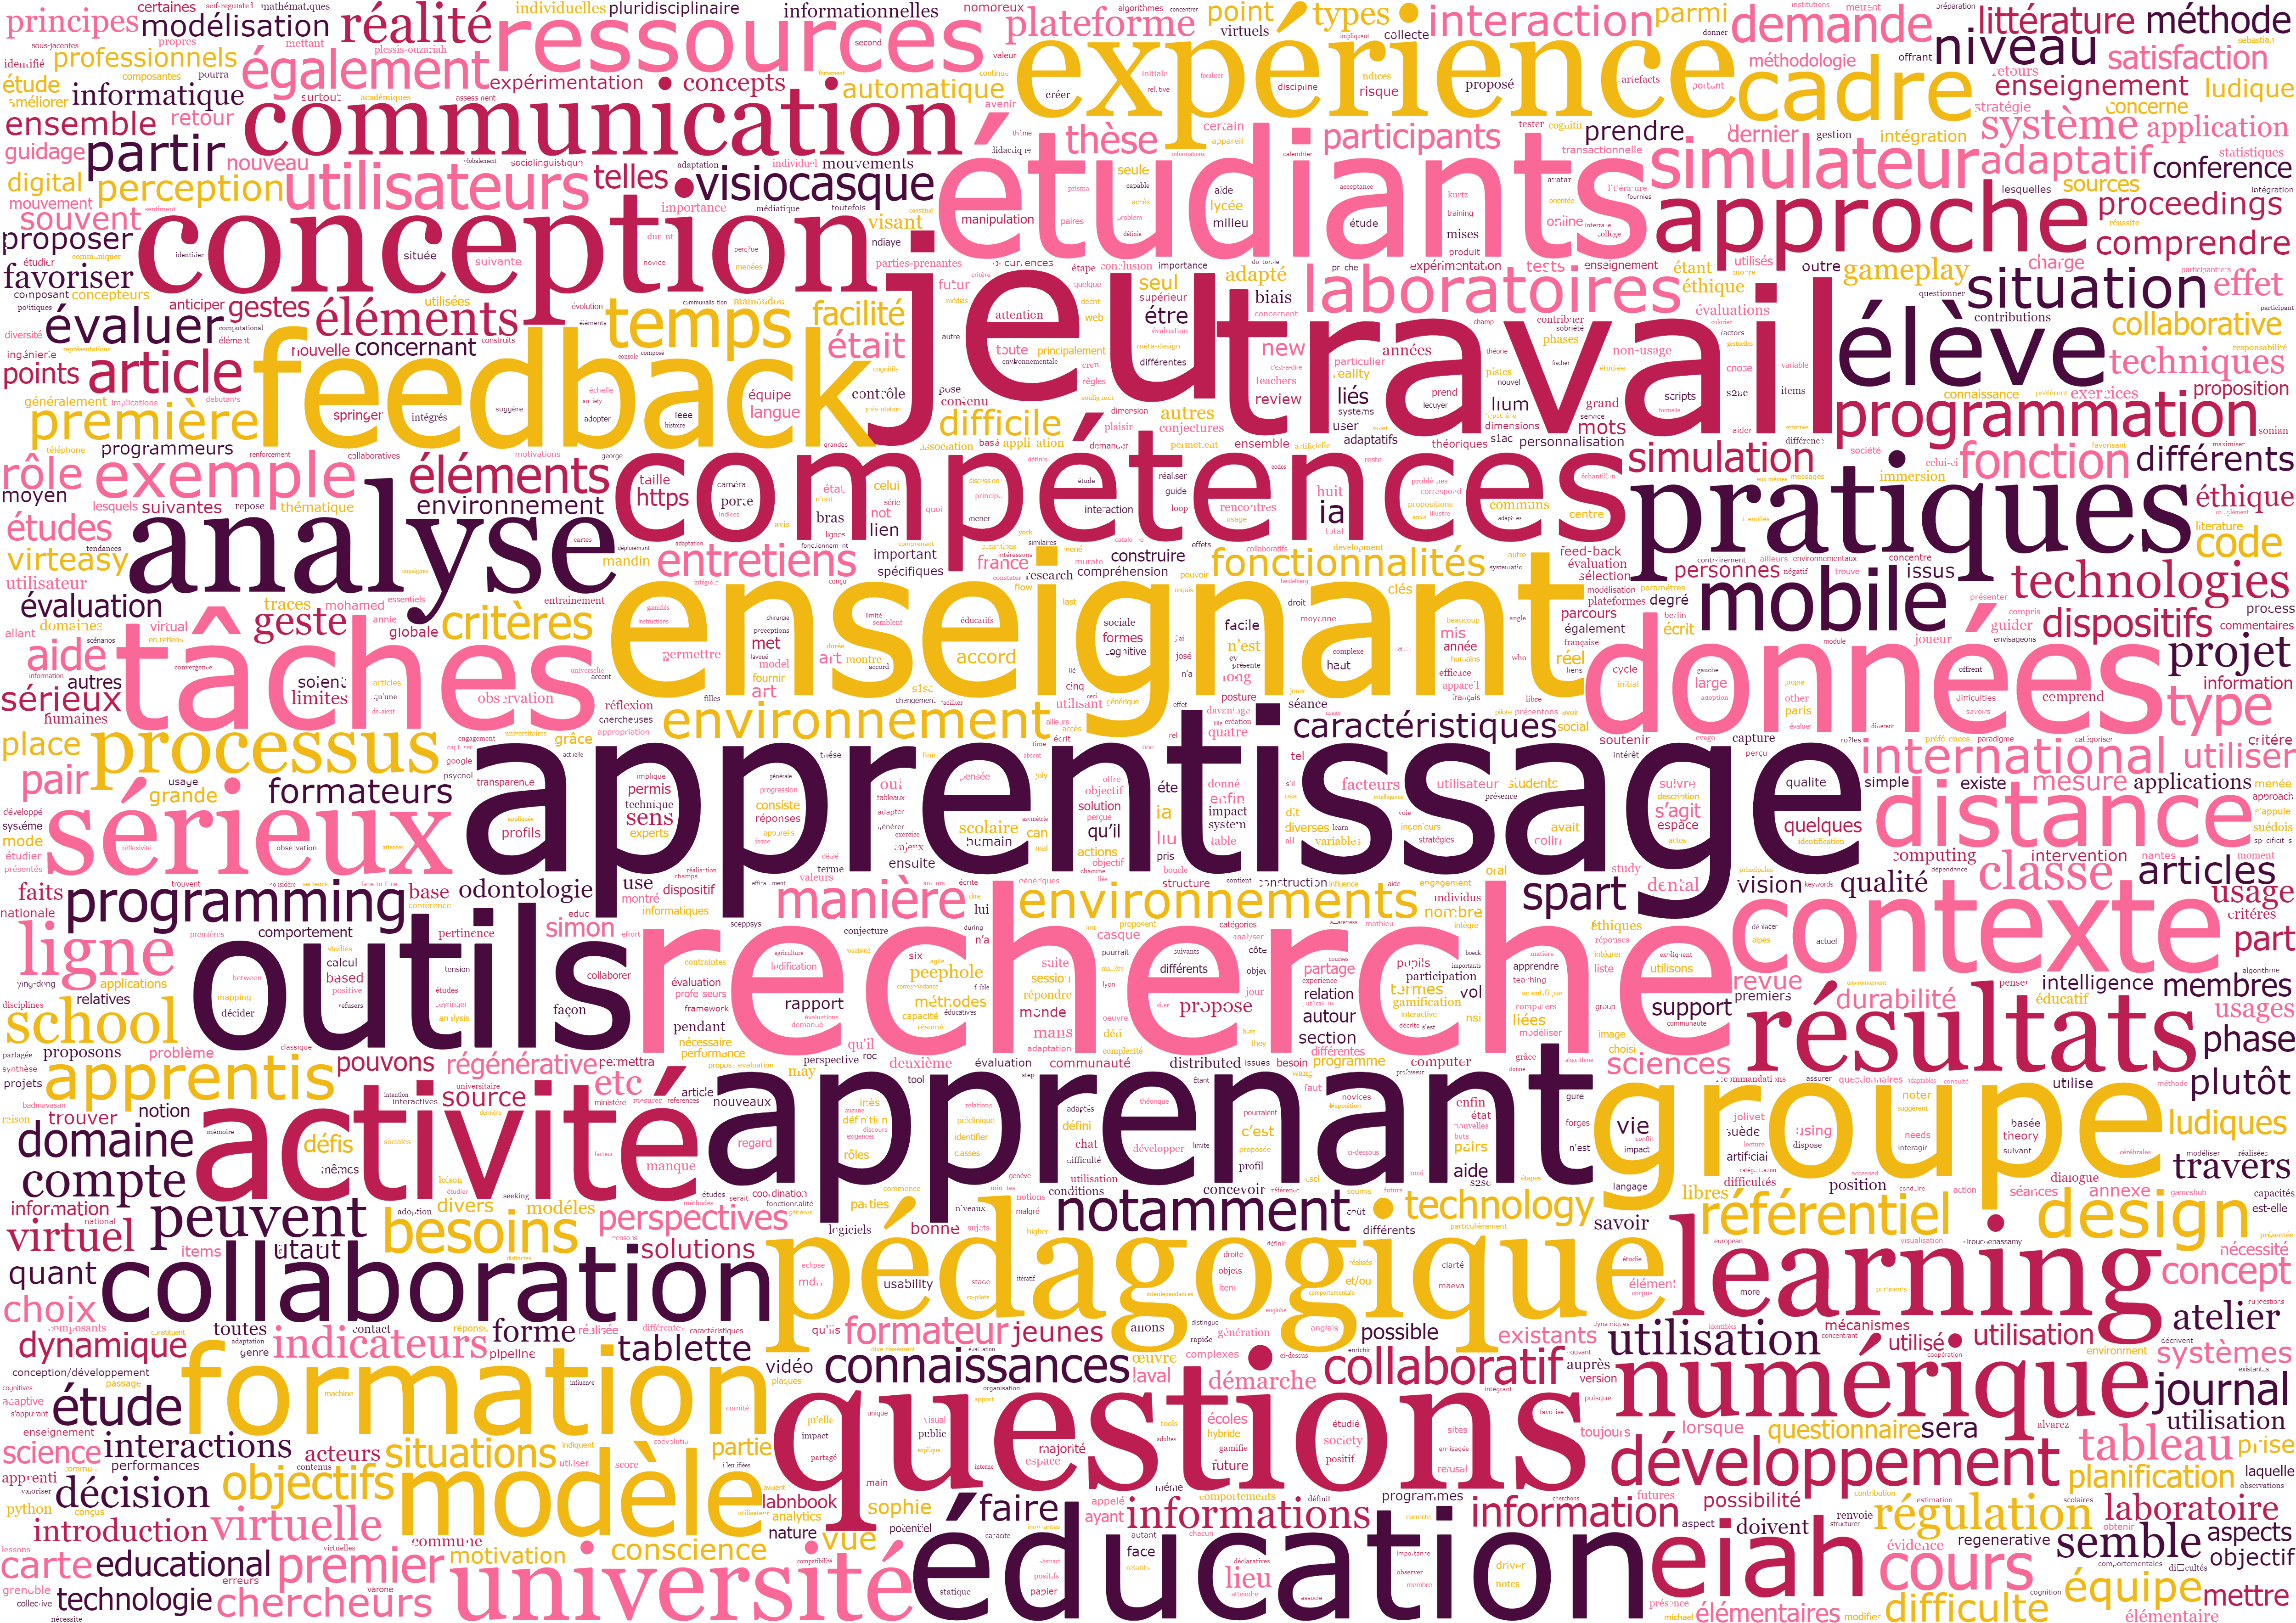
\includegraphics[width=0.7\textwidth]{Content/figures/wordcloud.png}
\end{figure}

\begin{center}
	\begin{Large}
		Édités par Catherine Bonnat et Rémi Venant
	\end{Large}

	\begin{large}
		Les 9 et 10 mai 2022\\
		Université de Lille\\
		France
	\end{large}
\end{center}

\vspace*{\fill}

\begin{figure}[!ht]
	\centering
	\includegraphics[width=.15\textwidth,valign=m]{Content/figures/atief.png}\hfill
	\includegraphics[width=.15\textwidth,valign=m]{Content/figures/cristal.png}\hfill
	\includegraphics[width=.15\textwidth,valign=m]{Content/figures/cirel.png}\hfill
\end{figure}

\noindent Avec le soutien de

\begin{figure}[!ht]
	\centering
	\includegraphics[width=.18\textwidth,valign=m]{Content/figures/regionHautDeFrance.jpg}\hfill
	\includegraphics[width=.18\textwidth,valign=m]{Content/figures/univLille.png}\hfill
	\includegraphics[width=.18\textwidth,valign=m]{Content/figures/interreg.png}\hfill
\end{figure}

\begin{center}
	\small{Les neuvièmes rencontres jeunes chercheur·e·s en EIAH 2022 ont été organisées par l’Université de Lille sous l’égide de l’ATIEF (Association des Technologies de l’Information pour l’Education et la Formation)}
\end{center}

\restoregeometry
\newpage